\section{数据预处理与结构特征分析}

\subsection{原始字段到计算依赖的转换}
本章的数据预处理与结构特征分析使用 OpenAI GPT-6（模型标识：gpt-6-astra；发布日期：2026 年 9 月 3 日）辅助梳理分析思路和结果表述\cite{AIGPT6}。表中统计量由项目脚本根据 100 张原始计算图计算；队伍核对数据来源、计算过程与解释。工具使用范围及人工复核责任见附录。

预处理按节点类型解析张量、计算操作和搬运操作，保留原始标识与字段。原始图在既有独立验收中通过附件的字段和图结构校验；本轮逐一核对 100 图 SHA256 与结构表记录一致。描述性统计读取原始字段，张量大小与操作周期均不重估，以便后续结果可追溯到同一输入。正式求解入口尚未覆盖的非法输入检查在第九章单列，不将离线数据核查等同于程序具备全部输入防护。

从操作集合中取出非 COPY 操作 $O_c$，经张量连接的生产与消费关系投影为
\begin{equation}
G_c=(O_c,E_c),\qquad
E_c=\{(u,v)\in O_c^2:\exists t\in T,\ (u,t),(t,v)\in E\}.
\label{eq:q1-opgraph}
\end{equation}
投影图用于判断操作先后及计算区域。张量标识、大小、生产者和消费者继续保存在索引表中，因此同一张量被多个操作消费时，可以按其实际共享关系计算搬运和驻留，而不把每条投影边都当作一份独立数据。原图中的 COPY 还用于识别输入读入与最终输出；投影不删除最终执行所需的搬运。

\subsection{面向调度的结构量}
对 $G_c$ 进行拓扑排序，并在其无向形式上提取弱连通分量 $\mathcal C=\{C_1,\ldots,C_K\}$。沿拓扑序计算深度与层宽，再累计各分量的双管道工作量：
\begin{equation}
\begin{aligned}
d_u&=1+\max_{v\in\operatorname{pred}(u)}d_v,\quad h=\max_u d_u,\\
m_\ell&=|\{u:d_u=\ell\}|,\qquad
W_j^q=\sum_{u\in C_j,\ p(u)=q}c_u,\quad q\in\{M,V\}.
\end{aligned}
\label{eq:q1-features}
\end{equation}
无前驱操作的深度为 1。入度大于 1 标识汇合位置，出度大于 1 标识分支位置。总工作量 $W=\sum_u c_u$ 与计算关键路径长度 $L$ 由
\begin{equation}
\lambda_u=c_u+\max_{v\in\operatorname{pred}(u)}\lambda_v,\qquad
L=\max_u\lambda_u,\qquad \rho=W/L
\label{eq:span}
\end{equation}
得到，空前驱的最大值取零。$\rho$ 描述忽略通信和资源竞争后的工作量与路径长度之比，用于观察潜在并行结构；它不等于本题实际可取得的加速比。

还统计最大分量操作数占比与向量工作量占比：
\[q_{\max}=\frac{\max_j|C_j|}{|O_c|},\qquad q_V=\frac{\sum_{p(u)=V}c_u}{W}.\]
此外，统计具有两个及以上非 COPY 消费者的外部输入张量数。$q_{\max}$ 按操作个数计算，与最大分量的周期占比不同。对于操作周期差异明显的图，后续装箱直接使用 $W_j^M,W_j^V$，不以节点个数代替负载。

\begin{table}[htbp]
\centering
\caption{100 个原始计算图的描述性统计}
\label{tab:inputstats}
\begin{tabular}{lrrr}
\hline
统计量 & 最小值 & 中位数 & 最大值 \\
\hline
非 COPY 操作数 & 552 & 3720.5 & 35705 \\
操作依赖边数 & 400 & 4017 & 38493 \\
弱连通分量数 $K$ & 1 & 39.5 & 2666 \\
拓扑深度 $h$ & 3 & 47.5 & 2440 \\
计算工作量 $W$/cycle & 23052 & 509952 & 61275840 \\
计算关键路径 $L$/cycle & 400 & 6140 & 863040 \\
工作量与路径比 $\rho$ & 3.42 & 43.13 & 6258.78 \\
\hline
\end{tabular}
\end{table}

\begin{figure}[htbp]
\centering
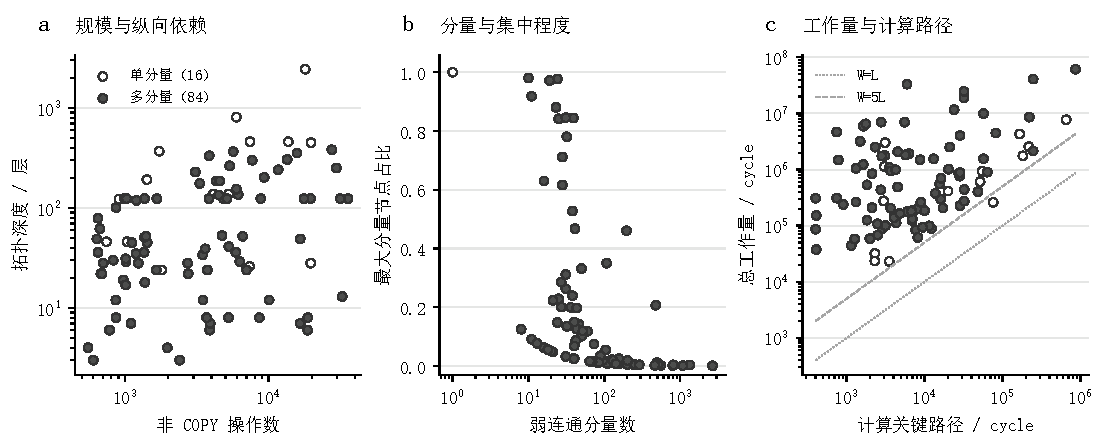
\includegraphics[width=\linewidth]{figures/fig5_1.pdf}
\caption{100 图的结构与工作量差异，每个点代表一张原始图。a 操作规模与拓扑深度；b 分量数与最大分量节点占比；c 计算关键路径与总工作量，参考线表示 $W=L$ 和 $W=5L$。空心、实心符号区分单分量和多分量图。对数坐标用于展示数量级跨度，不改变特征计算。}
\label{fig:inputstats}
\end{figure}

\subsection{特征如何进入三问决策}
84 个图具有多个弱连通分量，且其分量数均不少于 5；另有 16 个图只有一个分量。前一类通常提供直接分配独立计算块的机会，后一类若只保持分量完整，将无法利用多个核心。最大分量节点占比的中位数约为 0.122，也存在接近 1 的图，说明“分量很多”和“负载容易均衡”仍需分别判断。

共有 97 个图包含被多个计算操作消费的外部输入。这些输入是问题三共享读取的潜在来源，但它们也可能在同一核心内部完成复用，或因请求同时到达而无法命中 L2。此处统计仅用于识别可利用的数据关系；实际收益由第八章的事件模型及配对实验判断。

\begin{table}[htbp]
\centering
\caption{预处理特征与后续决策的对应关系}
\label{tab:featureuse}
\begin{tabular}{p{0.24\linewidth}p{0.29\linewidth}p{0.36\linewidth}}
\hline
原图信息 & 计算量 & 对应建模作用 \\
\hline
生产--消费依赖 & 分量、拓扑序、分支与汇合 & 第六章保留完整分量或选择内部切分位置 \\
操作周期与管道 & $W_j^M,W_j^V$ & 三问共用的双管道负载分配 \\
深度和层宽 & $h,m_\ell$、结构层间距 & 确定深度带尺度与层宽收缩边界 \\
张量大小与消费者 & 边界字节、跨核消费集合 & 第六、七章的搬运估计与同核复用 \\
存储位置与使用序列 & 活跃区间、峰值、下一次使用 & 第七、八章的 L1/UB 风险与换出估计 \\
共享输入与访问事件 & 读取先后、FIFO 驻留窗口 & 第八章的读路径选择与缓存收益解释 \\
\hline
\end{tabular}
\end{table}

结构特征在输入到达时重新提取。算法不把 100 图的均值、分位数或用例编号作为类别阈值；表~\ref{tab:inputstats} 和图~\ref{fig:inputstats} 用来解释输入差异，实际构造尺度由各图自身的深度、工作量及分支位置计算。这样的分工使数据分析与算法机理相互连接，同时保留了对新图进行结构分析的接口。
